\documentclass[12pt,a4 paper] {article}
\usepackage{graphicx}
\usepackage{amsmath}
\usepackage{amssymb}
\usepackage{fourier}
\usepackage{eulervm}
\title{S4\_VHDL Specifications}
\author{Nils Schlegel, 32067 \\ Tara Jaishi, 32289}
\date{06.11.2020}


\begin{document}
	\maketitle

\begin{figure}[h]
	\centering
	
\includegraphics[scale=0.4]{../png/hs.png}
	
\end{figure}
\newpage

\section{Product Overview - IC\_4 Top View}

History\\
\line(1,0){400}
\begin{flushleft}
	Target Spec. Current version: 0.1, 2020-11-9 \\
\hspace{2.2cm}	Previous version:-\\
\line(1,0){400}\\	             
\hspace{2.2cm}	06.11.2020 \hfill General description added\\
\hspace{2.2cm}	06.11.2020 \hfill Block diagram added\\
\hspace{2.2cm}	06.11.2020	\hfill Functional description added
\end{flushleft}

\subsection{General description}
IC4 is a single chip based application containing processing capabilities to detect and keep track of the amount of people in one room. It is part of a system solution to fullfill the covid-19-restrictions and regulate the amount of people in an area. This solution is only meant for a chamber with only one doorway available to enter or to exit.\newline
The IC4 is designed on a FPGA prototype-board Max1000 with 10M16SAU169C8G device on board.
\subsection{Block diagram}
\begin{figure}[h]
	\centering	
	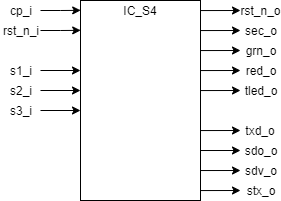
\includegraphics[scale=0.5]{../png/top.png}
\end{figure}
\newpage

\begin{center}
\begin{tabular}{llr}
Signal & Signal name & Description \\ \hline
rb\_i & reset & reset, active low \\
cp\_i & system clock & e.g. 10MHz \\
s1\_i & light\_curtain s1 & log1: something passes \\
s2\_i & light\_curtain s2 & log1: something passes \\
s3\_i & light\_curtain s3 & log1: something passes \\
grn\_o & LED, access garanted & Green LED, go ahead \\
red\_o & LED, stop, no entry & Red LED, stop, access denied \\
sdo\_o & serial data out & drives S3 or MC\\
sdv\_o & serial data valid & drives S3 or MC\\
stx\_o & serial transfer active & drives S3 or MC\\
txd\_o & serial out & to RS-232-driver, 9k6,8N2,ASCII,to PC\\
snd\_o & sound signal & acoustic signal, to loudspeaker\\
\\
inc\_s & increment & increments head count when triggered\\
dec\_s & decrement & decrements head count when triggered\\
num\_s &number & contains the head count number\\
evh\_s & event & contains the current event\\
\end{tabular}
\end{center}

\subsection{Functional description}
\subsection*{HeadCount}
Stores the current number of people in the room. It increments or decrements the number if needed.
\subsection*{EventHandler}
It recieves the signals from the light curtains and dectects with event is triggered. Depending on the event it will play a sound, turn on a LED and create an output signal.
\subsection*{UniqueTime}
This element is only counting the clock-cycles, to generate a unique timestamp. \newpage
\subsection*{UART}
The connection to RS232 is done by the UART. It takes the unique timestamp from the UART as well as the head count from the HeadCount and event type from the EventHandler, when a signal from the EventHandler is recieved.
\subsection*{3WireInterface}
The IC\_3 can be connected by using the 3WireInterface. When it recieves a signal from the EventHandler it should pass the head count and event type to the IC\_3.
\end{document}
	